\documentclass[]{article}
\usepackage{lmodern}
\usepackage{amssymb,amsmath}
\usepackage{ifxetex,ifluatex}
\usepackage{fixltx2e} % provides \textsubscript
\ifnum 0\ifxetex 1\fi\ifluatex 1\fi=0 % if pdftex
  \usepackage[T1]{fontenc}
  \usepackage[utf8]{inputenc}
\else % if luatex or xelatex
  \ifxetex
    \usepackage{mathspec}
  \else
    \usepackage{fontspec}
  \fi
  \defaultfontfeatures{Ligatures=TeX,Scale=MatchLowercase}
\fi
% use upquote if available, for straight quotes in verbatim environments
\IfFileExists{upquote.sty}{\usepackage{upquote}}{}
% use microtype if available
\IfFileExists{microtype.sty}{%
\usepackage{microtype}
\UseMicrotypeSet[protrusion]{basicmath} % disable protrusion for tt fonts
}{}
\usepackage[margin=1in]{geometry}
\usepackage{hyperref}
\hypersetup{unicode=true,
            pdftitle={MovieLens Rating Prediction Project},
            pdfauthor={Nabeel Khan},
            pdfborder={0 0 0},
            breaklinks=true}
\urlstyle{same}  % don't use monospace font for urls
\usepackage{color}
\usepackage{fancyvrb}
\newcommand{\VerbBar}{|}
\newcommand{\VERB}{\Verb[commandchars=\\\{\}]}
\DefineVerbatimEnvironment{Highlighting}{Verbatim}{commandchars=\\\{\}}
% Add ',fontsize=\small' for more characters per line
\usepackage{framed}
\definecolor{shadecolor}{RGB}{248,248,248}
\newenvironment{Shaded}{\begin{snugshade}}{\end{snugshade}}
\newcommand{\AlertTok}[1]{\textcolor[rgb]{0.94,0.16,0.16}{#1}}
\newcommand{\AnnotationTok}[1]{\textcolor[rgb]{0.56,0.35,0.01}{\textbf{\textit{#1}}}}
\newcommand{\AttributeTok}[1]{\textcolor[rgb]{0.77,0.63,0.00}{#1}}
\newcommand{\BaseNTok}[1]{\textcolor[rgb]{0.00,0.00,0.81}{#1}}
\newcommand{\BuiltInTok}[1]{#1}
\newcommand{\CharTok}[1]{\textcolor[rgb]{0.31,0.60,0.02}{#1}}
\newcommand{\CommentTok}[1]{\textcolor[rgb]{0.56,0.35,0.01}{\textit{#1}}}
\newcommand{\CommentVarTok}[1]{\textcolor[rgb]{0.56,0.35,0.01}{\textbf{\textit{#1}}}}
\newcommand{\ConstantTok}[1]{\textcolor[rgb]{0.00,0.00,0.00}{#1}}
\newcommand{\ControlFlowTok}[1]{\textcolor[rgb]{0.13,0.29,0.53}{\textbf{#1}}}
\newcommand{\DataTypeTok}[1]{\textcolor[rgb]{0.13,0.29,0.53}{#1}}
\newcommand{\DecValTok}[1]{\textcolor[rgb]{0.00,0.00,0.81}{#1}}
\newcommand{\DocumentationTok}[1]{\textcolor[rgb]{0.56,0.35,0.01}{\textbf{\textit{#1}}}}
\newcommand{\ErrorTok}[1]{\textcolor[rgb]{0.64,0.00,0.00}{\textbf{#1}}}
\newcommand{\ExtensionTok}[1]{#1}
\newcommand{\FloatTok}[1]{\textcolor[rgb]{0.00,0.00,0.81}{#1}}
\newcommand{\FunctionTok}[1]{\textcolor[rgb]{0.00,0.00,0.00}{#1}}
\newcommand{\ImportTok}[1]{#1}
\newcommand{\InformationTok}[1]{\textcolor[rgb]{0.56,0.35,0.01}{\textbf{\textit{#1}}}}
\newcommand{\KeywordTok}[1]{\textcolor[rgb]{0.13,0.29,0.53}{\textbf{#1}}}
\newcommand{\NormalTok}[1]{#1}
\newcommand{\OperatorTok}[1]{\textcolor[rgb]{0.81,0.36,0.00}{\textbf{#1}}}
\newcommand{\OtherTok}[1]{\textcolor[rgb]{0.56,0.35,0.01}{#1}}
\newcommand{\PreprocessorTok}[1]{\textcolor[rgb]{0.56,0.35,0.01}{\textit{#1}}}
\newcommand{\RegionMarkerTok}[1]{#1}
\newcommand{\SpecialCharTok}[1]{\textcolor[rgb]{0.00,0.00,0.00}{#1}}
\newcommand{\SpecialStringTok}[1]{\textcolor[rgb]{0.31,0.60,0.02}{#1}}
\newcommand{\StringTok}[1]{\textcolor[rgb]{0.31,0.60,0.02}{#1}}
\newcommand{\VariableTok}[1]{\textcolor[rgb]{0.00,0.00,0.00}{#1}}
\newcommand{\VerbatimStringTok}[1]{\textcolor[rgb]{0.31,0.60,0.02}{#1}}
\newcommand{\WarningTok}[1]{\textcolor[rgb]{0.56,0.35,0.01}{\textbf{\textit{#1}}}}
\usepackage{longtable,booktabs}
\usepackage{graphicx,grffile}
\makeatletter
\def\maxwidth{\ifdim\Gin@nat@width>\linewidth\linewidth\else\Gin@nat@width\fi}
\def\maxheight{\ifdim\Gin@nat@height>\textheight\textheight\else\Gin@nat@height\fi}
\makeatother
% Scale images if necessary, so that they will not overflow the page
% margins by default, and it is still possible to overwrite the defaults
% using explicit options in \includegraphics[width, height, ...]{}
\setkeys{Gin}{width=\maxwidth,height=\maxheight,keepaspectratio}
\IfFileExists{parskip.sty}{%
\usepackage{parskip}
}{% else
\setlength{\parindent}{0pt}
\setlength{\parskip}{6pt plus 2pt minus 1pt}
}
\setlength{\emergencystretch}{3em}  % prevent overfull lines
\providecommand{\tightlist}{%
  \setlength{\itemsep}{0pt}\setlength{\parskip}{0pt}}
\setcounter{secnumdepth}{5}
% Redefines (sub)paragraphs to behave more like sections
\ifx\paragraph\undefined\else
\let\oldparagraph\paragraph
\renewcommand{\paragraph}[1]{\oldparagraph{#1}\mbox{}}
\fi
\ifx\subparagraph\undefined\else
\let\oldsubparagraph\subparagraph
\renewcommand{\subparagraph}[1]{\oldsubparagraph{#1}\mbox{}}
\fi

%%% Use protect on footnotes to avoid problems with footnotes in titles
\let\rmarkdownfootnote\footnote%
\def\footnote{\protect\rmarkdownfootnote}

%%% Change title format to be more compact
\usepackage{titling}

% Create subtitle command for use in maketitle
\providecommand{\subtitle}[1]{
  \posttitle{
    \begin{center}\large#1\end{center}
    }
}

\setlength{\droptitle}{-2em}

  \title{MovieLens Rating Prediction Project}
    \pretitle{\vspace{\droptitle}\centering\huge}
  \posttitle{\par}
    \author{Nabeel Khan}
    \preauthor{\centering\large\emph}
  \postauthor{\par}
      \predate{\centering\large\emph}
  \postdate{\par}
    \date{16-May-2020}


\begin{document}
\maketitle

{
\setcounter{tocdepth}{2}
\tableofcontents
}
\section{Introduction} 
\label{sec:introduction}

This report is part of the `HarvardX: PH125.9x Data Science: Capstone'
course. The goal of this work is to use the acquired data science skills
to develop a recomender system.

\subsection{Background} 
\label{sec:background}

Recommender systems predict users' interests and recommend product items
that quite likely are interesting for them\cite{rsystems,systems1}.
These systems use state of the art machine learning algorithms to make
precise predictions. The recommender systems are most commonly used by
Netflix, YouTube, Spotify, Amazon, or Ebay.

One of the famous success story of the recommender system is the Netflix
competition\cite{nfc}. In 2006, Netflix announced to award 1 milloin
dollar prize to a team, which can come up with the best filtering
algorithm to predict user ratings for movies based on previous ratings.
The winners were announced in 2009 and the winning team improved the
accuracy of Netfliix system system by 10\%.

\subsection{Aim of Project} 
\label{sec:projectaim}

The aim of this project is to dveleop a recomender system using machine
learning to predict movie ratings based on suitable predictors.

\section{Dataset and Evaluation Metric} 
\label{sec:datasetmetric}

Netflix dataset is not available online. So, we will use 10M version of
MoiveLens dataset in this project \cite{dataset}. The dataset is
generated by the GroupLens, which is a research lab in the Department of
Computer Science and Engineering at the University of Minnesota. The
dataset contains 10 million ratings. We will split the data into
training and validaiton sets to develop the machine lelarning algorithm.

The performace of the model will be evaluated with the Root Mean Square
Error (RMSE) \cite{rmse}. The RMSE is a standard method to measure the
error of a model in predicting quantitative data and is defined in
Equation \ref{eq:rmse}.

\begin{equation}
\label{eq:rmse}
RMSE = \sqrt{\frac{1}{n}\displaystyle\sum_{i=1}^{n} (\hat{y}_{i}-y_{i})^{2}}
\end{equation}

\(\hat{y}_{i}\) refers to the predicted values by the model, \({y}_{i}\)
refers to the actual values, and \emph{n} refers to the total number of
oservations. The RMSE is one of the very useful metrics to analyse the
performance of models, but it can produce biased results in the presence
of large number of outliers. In this project, the RMSE will indicate how
close model predictions are to the actual ratings in the validation set.

\subsection{Download Data}
\label{datadownload}

After downloading data from the website, we split it into training set
referred to as \emph{edx} and test set referred to as \emph{validation}.
The \emph{edx} data consist of 90\% of the data, while 10\% of data is
used for validation.

\begin{itemize}
\item The model will be trained using \emph{edx} dataset and 
\emph{validation} dataset will be used to compute the RMSE.
\end{itemize}

\begin{Shaded}
\begin{Highlighting}[]
\CommentTok{################################}
\CommentTok{#  Install packages (if not installed)}
\CommentTok{################################}
\CommentTok{# Note: this process could take a couple of minutes}
\ControlFlowTok{if}\NormalTok{(}\OperatorTok{!}\KeywordTok{require}\NormalTok{(tidyverse)) }\KeywordTok{install.packages}\NormalTok{(}\StringTok{"tidyverse"}\NormalTok{, }\DataTypeTok{repos =} \StringTok{"http://cran.us.r-project.org"}\NormalTok{)}
\end{Highlighting}
\end{Shaded}

\begin{verbatim}
## Loading required package: tidyverse
\end{verbatim}

\begin{verbatim}
## -- Attaching packages --------------------------------------------------- tidyverse 1.3.0 --
\end{verbatim}

\begin{verbatim}
## v ggplot2 3.2.1     v purrr   0.3.3
## v tibble  2.1.3     v dplyr   0.8.3
## v tidyr   1.0.0     v stringr 1.4.0
## v readr   1.3.1     v forcats 0.4.0
\end{verbatim}

\begin{verbatim}
## -- Conflicts ------------------------------------------------------ tidyverse_conflicts() --
## x dplyr::filter() masks stats::filter()
## x dplyr::lag()    masks stats::lag()
\end{verbatim}

\begin{Shaded}
\begin{Highlighting}[]
\ControlFlowTok{if}\NormalTok{(}\OperatorTok{!}\KeywordTok{require}\NormalTok{(caret)) }\KeywordTok{install.packages}\NormalTok{(}\StringTok{"caret"}\NormalTok{, }\DataTypeTok{repos =} \StringTok{"http://cran.us.r-project.org"}\NormalTok{)}
\end{Highlighting}
\end{Shaded}

\begin{verbatim}
## Loading required package: caret
\end{verbatim}

\begin{verbatim}
## Loading required package: lattice
\end{verbatim}

\begin{verbatim}
## 
## Attaching package: 'caret'
\end{verbatim}

\begin{verbatim}
## The following object is masked from 'package:purrr':
## 
##     lift
\end{verbatim}

\begin{Shaded}
\begin{Highlighting}[]
\ControlFlowTok{if}\NormalTok{(}\OperatorTok{!}\KeywordTok{require}\NormalTok{(data.table)) }\KeywordTok{install.packages}\NormalTok{(}\StringTok{"data.table"}\NormalTok{, }\DataTypeTok{repos =} \StringTok{"http://cran.us.r-project.org"}\NormalTok{)}
\end{Highlighting}
\end{Shaded}

\begin{verbatim}
## Loading required package: data.table
\end{verbatim}

\begin{verbatim}
## 
## Attaching package: 'data.table'
\end{verbatim}

\begin{verbatim}
## The following objects are masked from 'package:dplyr':
## 
##     between, first, last
\end{verbatim}

\begin{verbatim}
## The following object is masked from 'package:purrr':
## 
##     transpose
\end{verbatim}

\begin{Shaded}
\begin{Highlighting}[]
\ControlFlowTok{if}\NormalTok{(}\OperatorTok{!}\KeywordTok{require}\NormalTok{(lubridate)) }\KeywordTok{install.packages}\NormalTok{(}\StringTok{"lubridate"}\NormalTok{, }\DataTypeTok{repos =} \StringTok{"http://cran.us.r-project.org"}\NormalTok{)}
\end{Highlighting}
\end{Shaded}

\begin{verbatim}
## Loading required package: lubridate
\end{verbatim}

\begin{verbatim}
## 
## Attaching package: 'lubridate'
\end{verbatim}

\begin{verbatim}
## The following objects are masked from 'package:data.table':
## 
##     hour, isoweek, mday, minute, month, quarter, second, wday,
##     week, yday, year
\end{verbatim}

\begin{verbatim}
## The following object is masked from 'package:base':
## 
##     date
\end{verbatim}

\begin{Shaded}
\begin{Highlighting}[]
\ControlFlowTok{if}\NormalTok{(}\OperatorTok{!}\KeywordTok{require}\NormalTok{(dplyr)) }\KeywordTok{install.packages}\NormalTok{(}\StringTok{"dplyr"}\NormalTok{, }\DataTypeTok{repos =} \StringTok{"http://cran.us.r-project.org"}\NormalTok{)}


\CommentTok{################################}
\CommentTok{# Load libraries}
\CommentTok{################################}
\KeywordTok{library}\NormalTok{(lubridate)}
\KeywordTok{library}\NormalTok{(tidyverse)}
\KeywordTok{library}\NormalTok{(dplyr)}
\KeywordTok{library}\NormalTok{(lubridate)}
\end{Highlighting}
\end{Shaded}

\begin{Shaded}
\begin{Highlighting}[]
\CommentTok{################################}
\CommentTok{# Downloading data}
\CommentTok{################################}
\CommentTok{# MovieLens 10M dataset:}
 \CommentTok{# https://grouplens.org/datasets/movielens/10m/}
 \CommentTok{# http://files.grouplens.org/datasets/movielens/ml-10m.zip}

\NormalTok{url <-}\StringTok{ "http://files.grouplens.org/datasets/movielens/ml-10m.zip"}

\NormalTok{dl <-}\StringTok{ }\KeywordTok{tempfile}\NormalTok{()}
    \KeywordTok{download.file}\NormalTok{(url, dl)}
  
\NormalTok{ratings <-}\StringTok{ }\KeywordTok{fread}\NormalTok{(}\DataTypeTok{text =} \KeywordTok{gsub}\NormalTok{(}\StringTok{"::"}\NormalTok{, }\StringTok{"}\CharTok{\textbackslash{}t}\StringTok{"}\NormalTok{, }\KeywordTok{readLines}\NormalTok{(}\KeywordTok{unzip}\NormalTok{(dl, }\StringTok{"ml-10M100K/ratings.dat"}\NormalTok{))), }\DataTypeTok{col.names =} \KeywordTok{c}\NormalTok{(}\StringTok{"userId"}\NormalTok{, }\StringTok{"movieId"}\NormalTok{, }\StringTok{"rating"}\NormalTok{, }\StringTok{"timestamp"}\NormalTok{))}
\NormalTok{movies <-}\StringTok{ }\KeywordTok{str_split_fixed}\NormalTok{(}\KeywordTok{readLines}\NormalTok{(}\KeywordTok{unzip}\NormalTok{(dl, }\StringTok{"ml-10M100K/movies.dat"}\NormalTok{)), }\StringTok{"}\CharTok{\textbackslash{}\textbackslash{}}\StringTok{::"}\NormalTok{, }\DecValTok{3}\NormalTok{)}
   \KeywordTok{colnames}\NormalTok{(movies) <-}\StringTok{ }\KeywordTok{c}\NormalTok{(}\StringTok{"movieId"}\NormalTok{, }\StringTok{"title"}\NormalTok{, }\StringTok{"genres"}\NormalTok{)}
\NormalTok{   movies <-}\StringTok{ }\KeywordTok{as.data.frame}\NormalTok{(movies) }\OperatorTok\StringTok{ }\KeywordTok{mutate}\NormalTok{(}\DataTypeTok{movieId =}   \KeywordTok{as.numeric}\NormalTok{(}\KeywordTok{levels}\NormalTok{(movieId))[movieId], }\DataTypeTok{title =} \KeywordTok{as.character}\NormalTok{(title), }\DataTypeTok{genres =}    \KeywordTok{as.character}\NormalTok{(genres))}

\CommentTok{################################}
\CommentTok{# Creating edx and validation sets}
\CommentTok{################################}
\NormalTok{movielens <-}\StringTok{ }\KeywordTok{left_join}\NormalTok{(ratings, movies, }\DataTypeTok{by =} \StringTok{"movieId"}\NormalTok{)}


\CommentTok{# Validation set will be 10% of MovieLens data}
\KeywordTok{set.seed}\NormalTok{(}\DecValTok{1}\NormalTok{, }\DataTypeTok{sample.kind =} \StringTok{"Rounding"}\NormalTok{)}
\end{Highlighting}
\end{Shaded}

\begin{verbatim}
## Warning in set.seed(1, sample.kind = "Rounding"): non-uniform 'Rounding'
## sampler used
\end{verbatim}

\begin{Shaded}
\begin{Highlighting}[]
\NormalTok{test_index <-}\StringTok{ }\KeywordTok{createDataPartition}\NormalTok{(}\DataTypeTok{y =}\NormalTok{ movielens}\OperatorTok{$}\NormalTok{rating, }\DataTypeTok{times =} \DecValTok{1}\NormalTok{, }\DataTypeTok{p =} \FloatTok{0.1}\NormalTok{, }\DataTypeTok{list =} \OtherTok{FALSE}\NormalTok{)}

\NormalTok{edx <-}\StringTok{ }\NormalTok{movielens[}\OperatorTok{-}\NormalTok{test_index,]}
\NormalTok{temp <-}\StringTok{ }\NormalTok{movielens[test_index,]}

\CommentTok{# Make sure userId and movieId in validation set are also in edx set}
\NormalTok{validation <-}\StringTok{ }\NormalTok{temp }\OperatorTok\StringTok{ }
\StringTok{      }\KeywordTok{semi_join}\NormalTok{(edx, }\DataTypeTok{by =} \StringTok{"movieId"}\NormalTok{) }\OperatorTok
\StringTok{      }\KeywordTok{semi_join}\NormalTok{(edx, }\DataTypeTok{by =} \StringTok{"userId"}\NormalTok{)}

\CommentTok{# Add rows removed from validation set back into edx set}
\NormalTok{removed <-}\StringTok{ }\KeywordTok{anti_join}\NormalTok{(temp, validation)}
\end{Highlighting}
\end{Shaded}

\begin{verbatim}
## Joining, by = c("userId", "movieId", "rating", "timestamp", "title", "genres")
\end{verbatim}

\begin{Shaded}
\begin{Highlighting}[]
\NormalTok{ edx <-}\StringTok{ }\KeywordTok{rbind}\NormalTok{(edx, removed)}

 \CommentTok{# Removing the objects no longer required}
\KeywordTok{rm}\NormalTok{(dl, ratings, movies, test_index, temp, movielens, removed)}
\end{Highlighting}
\end{Shaded}

\section{Data Exploration}
\label{sec:dataanalysis}

In this section, we explore the dataset to get familiar with it. We also
also perform some data wrangling. Data wrangling is the process of
cleaning, structuring or enriching raw data into a desired format to
make better decisions and get more meaningful insights.

We look at the first six rows of \emph{edx} dataset. We can see that
dataset contains six variables namely
\texttt{userID\textquotesingle{}\textquotesingle{},}movieID'`,
\texttt{rating\textquotesingle{}\textquotesingle{},}timestamp'`,
\texttt{title\textquotesingle{}\textquotesingle{},\ and}genres''. Each
row represents a single rating of a user for a single movie.

\begin{Shaded}
\begin{Highlighting}[]
\KeywordTok{head}\NormalTok{(edx)}
\end{Highlighting}
\end{Shaded}

\begin{longtable}[]{@{}lrrrrll@{}}
\toprule
& userId & movieId & rating & timestamp & title & genres\tabularnewline
\midrule
\endhead
1 & 1 & 122 & 5 & 838985046 & Boomerang (1992) &
Comedy\textbar Romance\tabularnewline
2 & 1 & 185 & 5 & 838983525 & Net, The (1995) &
Action\textbar Crime\textbar Thriller\tabularnewline
4 & 1 & 292 & 5 & 838983421 & Outbreak (1995) &
Action\textbar Drama\textbar Sci-Fi\textbar Thriller\tabularnewline
5 & 1 & 316 & 5 & 838983392 & Stargate (1994) &
Action\textbar Adventure\textbar Sci-Fi\tabularnewline
6 & 1 & 329 & 5 & 838983392 & Star Trek: Generations (1994) &
Action\textbar Adventure\textbar Drama\textbar Sci-Fi\tabularnewline
7 & 1 & 355 & 5 & 838984474 & Flintstones, The (1994) &
Children\textbar Comedy\textbar Fantasy\tabularnewline
\bottomrule
\end{longtable}

There are around nine million rows in \emph{edx} dataset, which is
around 90\% of the whole data.

\begin{Shaded}
\begin{Highlighting}[]
\KeywordTok{sprintf}\NormalTok{(}\StringTok{"Edx Dataset - Rows = %d  | Columns = %d"}\NormalTok{,}\KeywordTok{nrow}\NormalTok{(edx),}\KeywordTok{ncol}\NormalTok{(edx))}
\end{Highlighting}
\end{Shaded}

\begin{verbatim}
## [1] "Edx Dataset - Rows = 9000055  | Columns = 6"
\end{verbatim}

The summary of \emph{edx} dataset indicates that there are no null
values. So, we don't need to perform any data cleaning.

\begin{Shaded}
\begin{Highlighting}[]
\KeywordTok{summary}\NormalTok{(edx)}
\end{Highlighting}
\end{Shaded}

\begin{verbatim}
##      userId         movieId          rating        timestamp        
##  Min.   :    1   Min.   :    1   Min.   :0.500   Min.   :7.897e+08  
##  1st Qu.:18124   1st Qu.:  648   1st Qu.:3.000   1st Qu.:9.468e+08  
##  Median :35738   Median : 1834   Median :4.000   Median :1.035e+09  
##  Mean   :35870   Mean   : 4122   Mean   :3.512   Mean   :1.033e+09  
##  3rd Qu.:53607   3rd Qu.: 3626   3rd Qu.:4.000   3rd Qu.:1.127e+09  
##  Max.   :71567   Max.   :65133   Max.   :5.000   Max.   :1.231e+09  
##     title              genres         
##  Length:9000055     Length:9000055    
##  Class :character   Class :character  
##  Mode  :character   Mode  :character  
##                                       
##                                       
## 
\end{verbatim}

\subsection{Data Wrangling}
\label{sec:dw}

The \emph{edx} dataset has a couple of issues:

\begin{enumerate}
\item The \emph{``title''} of each movie has its premier year appended to it.
\item The \emph{``timestamp''} contains the date on which user added his rating. But, the column shows the number of seconds that have elapsed since January 1, 1970.  
\end{enumerate}

To resolve these issues, we perform the following operations on both
training and validation datasets:

\begin{enumerate}
\item Create a new column \emph{``premiereYr''}, which will store the premier year of the movie. We strip out the year information from \emph{``title''} column.
\item Modify the \emph{``timestamp"} so that it contains the information in date format, which is easy to interprete. 
\end{enumerate}

The summary of \emph{edx} dataset shows that we have successfully
performed data wrangling operations.

\begin{Shaded}
\begin{Highlighting}[]
\CommentTok{#####################################}
\CommentTok{# EDX Dataset}
\CommentTok{#####################################}
\CommentTok{# Extracting premier date from movie title}
\NormalTok{edx <-edx }\OperatorTok\StringTok{ }\KeywordTok{extract}\NormalTok{(title, }\KeywordTok{c}\NormalTok{(}\StringTok{"title"}\NormalTok{, }\StringTok{"premiereYr"}\NormalTok{), }
                      \DataTypeTok{regex =} \StringTok{"^(.*) }\CharTok{\textbackslash{}\textbackslash{}}\StringTok{(([0-9 ##}\CharTok{\textbackslash{}\textbackslash{}}\StringTok{-]*)}\CharTok{\textbackslash{}\textbackslash{}}\StringTok{)$"}\NormalTok{)}
\NormalTok{edx}\OperatorTok{$}\NormalTok{premiereYr <-}\StringTok{ }\KeywordTok{as.numeric}\NormalTok{(edx}\OperatorTok{$}\NormalTok{premiereYr)}

\CommentTok{# Converting timestamp to date format}
\NormalTok{edx}\OperatorTok{$}\NormalTok{timestamp <-}\StringTok{ }\KeywordTok{as.Date}\NormalTok{(}\KeywordTok{as_datetime}\NormalTok{((edx}\OperatorTok{$}\NormalTok{timestamp), }\DataTypeTok{origin=}\StringTok{"1970-01-01"}\NormalTok{))}

\CommentTok{#####################################}
\CommentTok{# Validation Dataset}
\CommentTok{#####################################}
\CommentTok{# Extracting premier date from movie title}
\NormalTok{validation <-validation }\OperatorTok\StringTok{ }\KeywordTok{extract}\NormalTok{(title, }\KeywordTok{c}\NormalTok{(}\StringTok{"title"}\NormalTok{, }\StringTok{"premiereYr"}\NormalTok{),}
                                    \DataTypeTok{regex =} \StringTok{"^(.*) }\CharTok{\textbackslash{}\textbackslash{}}\StringTok{(([0-9 ##}\CharTok{\textbackslash{}\textbackslash{}}\StringTok{-]*)}\CharTok{\textbackslash{}\textbackslash{}}\StringTok{)$"}\NormalTok{)}
\NormalTok{validation}\OperatorTok{$}\NormalTok{premiereYr <-}\StringTok{ }\KeywordTok{as.numeric}\NormalTok{(validation}\OperatorTok{$}\NormalTok{premiereYr)}

\CommentTok{# Converting timestamp to date format}
\NormalTok{validation}\OperatorTok{$}\NormalTok{timestamp <-}\StringTok{ }\KeywordTok{as.Date}\NormalTok{(}\KeywordTok{as_datetime}\NormalTok{((validation}\OperatorTok{$}\NormalTok{timestamp), }\DataTypeTok{origin=}\StringTok{"1970-01-01"}\NormalTok{))}

\KeywordTok{head}\NormalTok{(edx)}
\end{Highlighting}
\end{Shaded}

\begin{longtable}[]{@{}lrrrllrl@{}}
\toprule
& userId & movieId & rating & timestamp & title & premiereYr &
genres\tabularnewline
\midrule
\endhead
1 & 1 & 122 & 5 & 1996-08-02 & Boomerang & 1992 &
Comedy\textbar Romance\tabularnewline
2 & 1 & 185 & 5 & 1996-08-02 & Net, The & 1995 &
Action\textbar Crime\textbar Thriller\tabularnewline
4 & 1 & 292 & 5 & 1996-08-02 & Outbreak & 1995 &
Action\textbar Drama\textbar Sci-Fi\textbar Thriller\tabularnewline
5 & 1 & 316 & 5 & 1996-08-02 & Stargate & 1994 &
Action\textbar Adventure\textbar Sci-Fi\tabularnewline
6 & 1 & 329 & 5 & 1996-08-02 & Star Trek: Generations & 1994 &
Action\textbar Adventure\textbar Drama\textbar Sci-Fi\tabularnewline
7 & 1 & 355 & 5 & 1996-08-02 & Flintstones, The & 1994 &
Children\textbar Comedy\textbar Fantasy\tabularnewline
\bottomrule
\end{longtable}

\section{Data Analysis}
\label{sec:dataanalysis}

In the previous section, we understood the structure of the data and
performed a couple of operations. In this section, we extract insights
about all features of the \emph{edx} dataset.

\subsection{Users}
\label{sec:users}

The dataset has around 69800 unique users. Each user can rate more than
one movie. If we look at the frequency of ratings for users, we can see
that the distribution is rightly skewed. Most of the users rate few
movies as shown in the graph. So, we can include a user penalty term in
our model (if needed) to improve the RMSE. The process of adding penatly
terms to error functions is known as \textbf{Regularization}
\cite{rafa}.

Regularization permits to penalize large estimates that are formed using
small sample sizes and avoids overfitting of data. The overfitting
occurs because model is trying too hard to capture the noise in the
training dataset. The basic idea behind regularization is to constrain
the total variability of the effect sizes.

\begin{Shaded}
\begin{Highlighting}[]
\NormalTok{edx }\OperatorTok
\KeywordTok{summarize}\NormalTok{(}\DataTypeTok{users =} \KeywordTok{n_distinct}\NormalTok{(userId))}
\end{Highlighting}
\end{Shaded}

\begin{longtable}[]{@{}r@{}}
\toprule
users\tabularnewline
\midrule
\endhead
69878\tabularnewline
\bottomrule
\end{longtable}

\begin{Shaded}
\begin{Highlighting}[]
\NormalTok{edx }\OperatorTok
\StringTok{  }\KeywordTok{count}\NormalTok{(userId) }\OperatorTok
\StringTok{  }\KeywordTok{ggplot}\NormalTok{(}\KeywordTok{aes}\NormalTok{(n)) }\OperatorTok{+}
\StringTok{  }\KeywordTok{geom_histogram}\NormalTok{(}\DataTypeTok{bins =} \DecValTok{30}\NormalTok{,  }\DataTypeTok{fill=}\StringTok{'cadetblue'}\NormalTok{, }\DataTypeTok{color=}\StringTok{'black'}\NormalTok{) }\OperatorTok{+}
\StringTok{  }\KeywordTok{scale_x_log10}\NormalTok{() }\OperatorTok{+}
\StringTok{  }\KeywordTok{xlab}\NormalTok{(}\StringTok{"Number of users"}\NormalTok{) }\OperatorTok{+}\StringTok{ }
\StringTok{  }\KeywordTok{ylab}\NormalTok{(}\StringTok{"Fequency of ratings"}\NormalTok{) }\OperatorTok{+}
\StringTok{  }\KeywordTok{ggtitle}\NormalTok{(}\StringTok{"Number of ratings given by Users"}\NormalTok{)}
\end{Highlighting}
\end{Shaded}

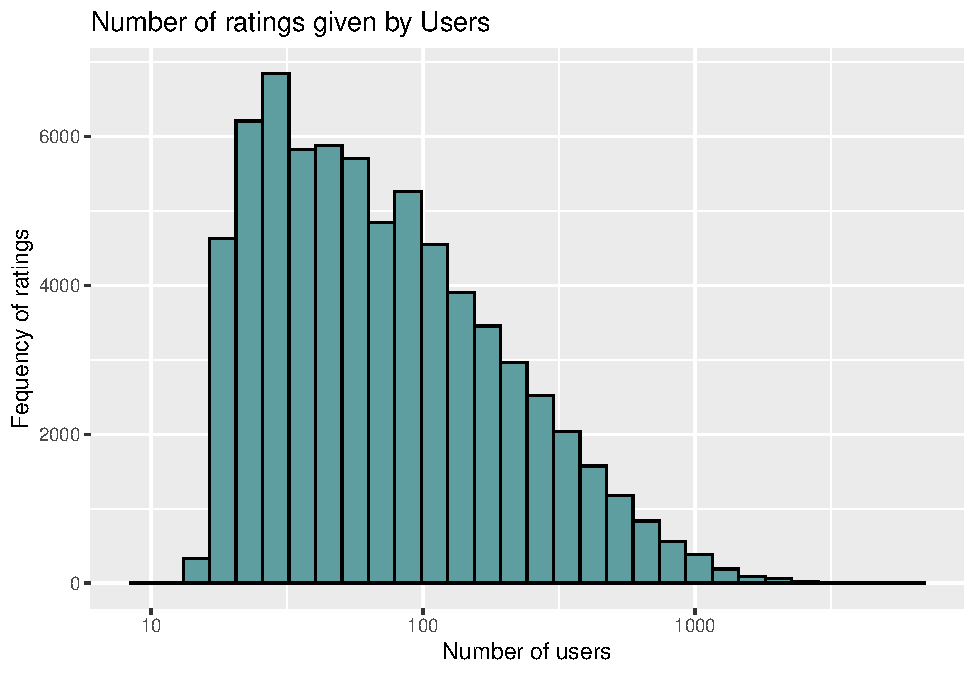
\includegraphics{Project_MovieLens_files/figure-latex/unnamed-chunk-8-1.pdf}

\subsection{Movies}

The dataset has around 10400 unique movies.

\begin{Shaded}
\begin{Highlighting}[]
\NormalTok{edx }\OperatorTok
\KeywordTok{summarize}\NormalTok{(}\DataTypeTok{users =} \KeywordTok{n_distinct}\NormalTok{(title))}
\end{Highlighting}
\end{Shaded}

\begin{longtable}[]{@{}r@{}}
\toprule
users\tabularnewline
\midrule
\endhead
10407\tabularnewline
\bottomrule
\end{longtable}

The release years for movies in \emph{edx} range 1915 to 2008. Most
movies belong to recent years ranging from 1980 to 2000. Though, it
would be nice to have more movies from old years to make model more
robust.

\begin{Shaded}
\begin{Highlighting}[]
\NormalTok{edx }\OperatorTok
\StringTok{  }\KeywordTok{select}\NormalTok{(movieId, premiereYr) }\OperatorTok\StringTok{ }\CommentTok{# select columns we need}
\StringTok{  }\KeywordTok{group_by}\NormalTok{(premiereYr) }\OperatorTok\StringTok{ }\CommentTok{# group by year}
\StringTok{  }\KeywordTok{summarise}\NormalTok{(}\DataTypeTok{count =} \KeywordTok{n}\NormalTok{())  }\OperatorTok\StringTok{ }\CommentTok{# count movies per year}
\StringTok{  }\KeywordTok{arrange}\NormalTok{(premiereYr)}\OperatorTok
\StringTok{  }\KeywordTok{ggplot}\NormalTok{(}\KeywordTok{aes}\NormalTok{(}\DataTypeTok{x =}\NormalTok{ premiereYr, }\DataTypeTok{y =}\NormalTok{ count)) }\OperatorTok{+}
\StringTok{  }\KeywordTok{geom_point}\NormalTok{(}\DataTypeTok{color=}\StringTok{"cadetblue"}\NormalTok{)}
\end{Highlighting}
\end{Shaded}

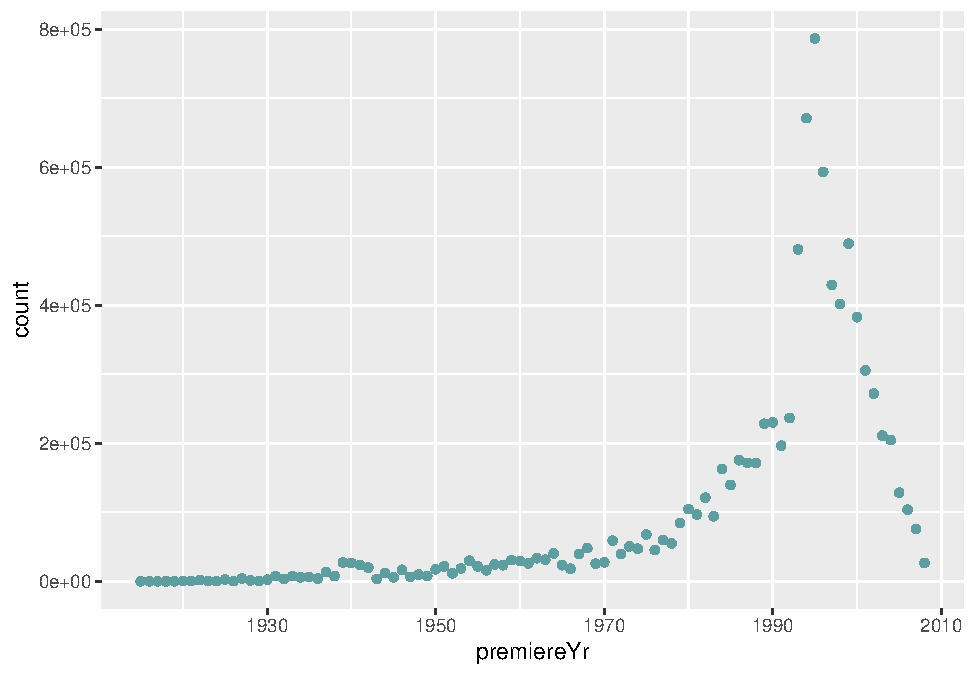
\includegraphics{Project_MovieLens_files/figure-latex/unnamed-chunk-10-1.pdf}

\begin{Shaded}
\begin{Highlighting}[]
\KeywordTok{hist}\NormalTok{(edx}\OperatorTok{$}\NormalTok{premiereYr, }\DataTypeTok{main=}\StringTok{"Release years of movies"}\NormalTok{)}
\end{Highlighting}
\end{Shaded}

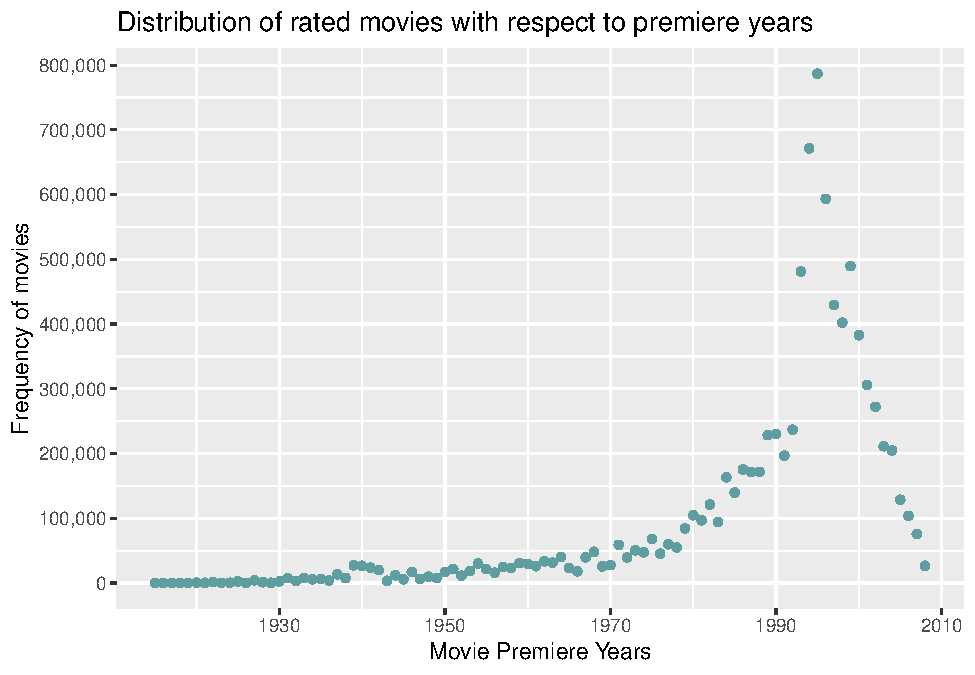
\includegraphics{Project_MovieLens_files/figure-latex/unnamed-chunk-11-1.pdf}
The distribution of ratings for movies indicate that most movies get a
decent number of ratings. Although some movies have less number fof
ratings.This indicates that movie information can also be used as
penalty term (if required).

\begin{Shaded}
\begin{Highlighting}[]
\CommentTok{#Distribution of Movie Ratings}
\NormalTok{edx }\OperatorTok\StringTok{ }\KeywordTok{group_by}\NormalTok{(movieId) }\OperatorTok\StringTok{ }\KeywordTok{summarize}\NormalTok{(}\DataTypeTok{n =} \KeywordTok{n}\NormalTok{()) }\OperatorTok
\StringTok{  }\KeywordTok{ggplot}\NormalTok{(}\KeywordTok{aes}\NormalTok{(n)) }\OperatorTok{+}\StringTok{ }\KeywordTok{geom_histogram}\NormalTok{(}\DataTypeTok{bins=}\DecValTok{30}\NormalTok{, }\DataTypeTok{fill =} \StringTok{'cadetblue'}\NormalTok{, }\DataTypeTok{color =} \StringTok{'black'}\NormalTok{) }\OperatorTok{+}
\StringTok{  }\KeywordTok{scale_x_log10}\NormalTok{() }\OperatorTok{+}
\StringTok{  }\KeywordTok{xlab}\NormalTok{(}\StringTok{"Number of movies"}\NormalTok{) }\OperatorTok{+}\StringTok{ }
\StringTok{  }\KeywordTok{ylab}\NormalTok{(}\StringTok{"Fequency of ratings"}\NormalTok{) }\OperatorTok{+}
\StringTok{  }\KeywordTok{ggtitle}\NormalTok{(}\StringTok{"Number of ratings per movie"}\NormalTok{)}
\end{Highlighting}
\end{Shaded}

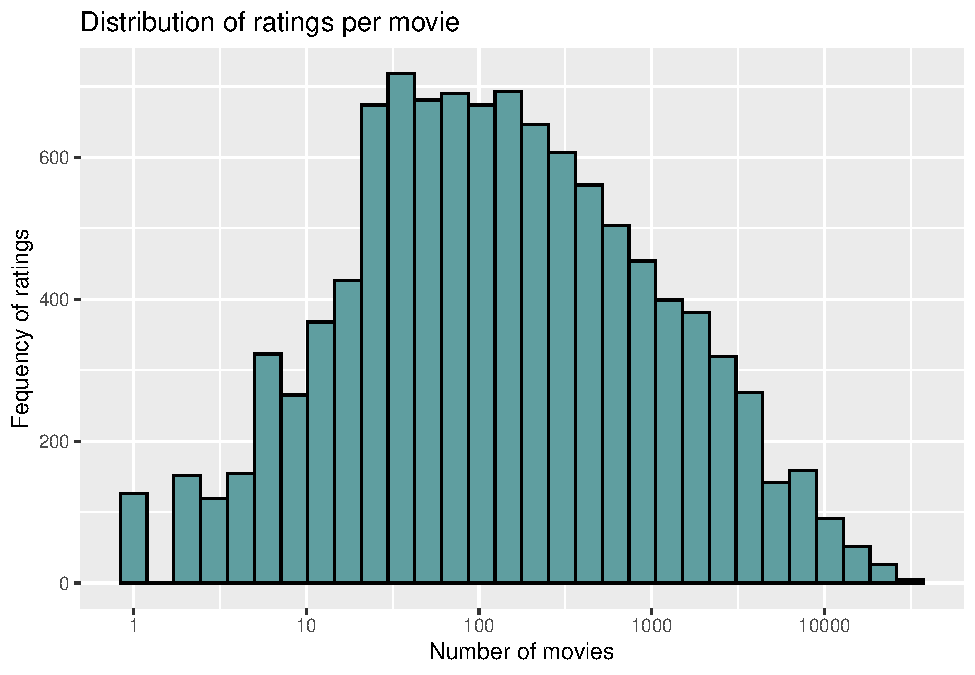
\includegraphics{Project_MovieLens_files/figure-latex/unnamed-chunk-12-1.pdf}

\subsection{Ratings}
\label{sec:ratings}

We observe that ratings data is collected over a span of around 14
years. All movies have at-least one rating. We also observe that there
is a tendency that users generally rate movies 3 or 4.

\begin{Shaded}
\begin{Highlighting}[]
\NormalTok{years<-}\KeywordTok{format}\NormalTok{(edx}\OperatorTok{$}\NormalTok{timestamp, }\DataTypeTok{format=}\StringTok{"%Y"}\NormalTok{)}
\KeywordTok{as.numeric}\NormalTok{(}\KeywordTok{max}\NormalTok{(years))}\OperatorTok{-}\KeywordTok{as.numeric}\NormalTok{(}\KeywordTok{min}\NormalTok{(years))}
\end{Highlighting}
\end{Shaded}

\begin{verbatim}
## [1] 14
\end{verbatim}

The movies can have half or full stars ratings. The distribution
indicates that most movies get full star ratings.

\begin{Shaded}
\begin{Highlighting}[]
\KeywordTok{print}\NormalTok{(}\StringTok{"Frequencies of ratings"}\NormalTok{)}
\end{Highlighting}
\end{Shaded}

\begin{verbatim}
## [1] "Frequencies of ratings"
\end{verbatim}

\begin{Shaded}
\begin{Highlighting}[]
\KeywordTok{sort}\NormalTok{(}\KeywordTok{table}\NormalTok{(edx}\OperatorTok{$}\NormalTok{rating))}
\end{Highlighting}
\end{Shaded}

\begin{verbatim}
## 
##     0.5     1.5     2.5       1     4.5       2     3.5       5       3 
##   85374  106426  333010  345679  526736  711422  791624 1390114 2121240 
##       4 
## 2588430
\end{verbatim}

\begin{Shaded}
\begin{Highlighting}[]
\CommentTok{# Generating groups of data for half star and full star ratings}
\NormalTok{group <-}\StringTok{  }\KeywordTok{ifelse}\NormalTok{((edx}\OperatorTok{$}\NormalTok{rating }\OperatorTok{==}\StringTok{ }\DecValTok{1} \OperatorTok{|}\NormalTok{edx}\OperatorTok{$}\NormalTok{rating }\OperatorTok{==}\StringTok{ }\DecValTok{2} \OperatorTok{|}\StringTok{ }\NormalTok{edx}\OperatorTok{$}\NormalTok{rating }\OperatorTok{==}\StringTok{ }\DecValTok{3} \OperatorTok{|}\StringTok{ }
\StringTok{                  }\NormalTok{edx}\OperatorTok{$}\NormalTok{rating }\OperatorTok{==}\StringTok{ }\DecValTok{4} \OperatorTok{|}\StringTok{ }\NormalTok{edx}\OperatorTok{$}\NormalTok{rating }\OperatorTok{==}\StringTok{ }\DecValTok{5}\NormalTok{) ,}
                   \StringTok{"whole_star"}\NormalTok{, }
                   \StringTok{"half_star"}\NormalTok{) }

\CommentTok{# Plotting the distribution of ratings}
\NormalTok{ratings_distribution <-}\StringTok{ }\KeywordTok{data.frame}\NormalTok{(edx}\OperatorTok{$}\NormalTok{rating, group)}
\KeywordTok{ggplot}\NormalTok{(ratings_distribution, }\KeywordTok{aes}\NormalTok{(}\DataTypeTok{x=}\NormalTok{ edx.rating, }\DataTypeTok{fill =}\NormalTok{ group)) }\OperatorTok{+}
\StringTok{  }\KeywordTok{geom_histogram}\NormalTok{( }\DataTypeTok{binwidth =} \FloatTok{0.2}\NormalTok{,}\DataTypeTok{color =} \StringTok{'black'}\NormalTok{) }\OperatorTok{+}
\StringTok{  }\KeywordTok{scale_x_discrete}\NormalTok{(}\DataTypeTok{limits =} \KeywordTok{c}\NormalTok{(}\KeywordTok{seq}\NormalTok{(}\FloatTok{0.5}\NormalTok{,}\DecValTok{5}\NormalTok{,}\FloatTok{0.5}\NormalTok{))) }\OperatorTok{+}
\StringTok{  }\KeywordTok{scale_y_continuous}\NormalTok{(}\DataTypeTok{breaks =} \KeywordTok{c}\NormalTok{(}\KeywordTok{seq}\NormalTok{(}\DecValTok{0}\NormalTok{, }\DecValTok{3000000}\NormalTok{, }\DecValTok{500000}\NormalTok{)))}\OperatorTok{+}
\StringTok{  }\KeywordTok{labs}\NormalTok{(}\DataTypeTok{x=}\StringTok{"Ratings"}\NormalTok{, }\DataTypeTok{y=}\StringTok{"Number of ratings"}\NormalTok{) }\OperatorTok{+}
\StringTok{  }\KeywordTok{ggtitle}\NormalTok{(}\StringTok{"Distribution of ratings"}\NormalTok{)}
\end{Highlighting}
\end{Shaded}

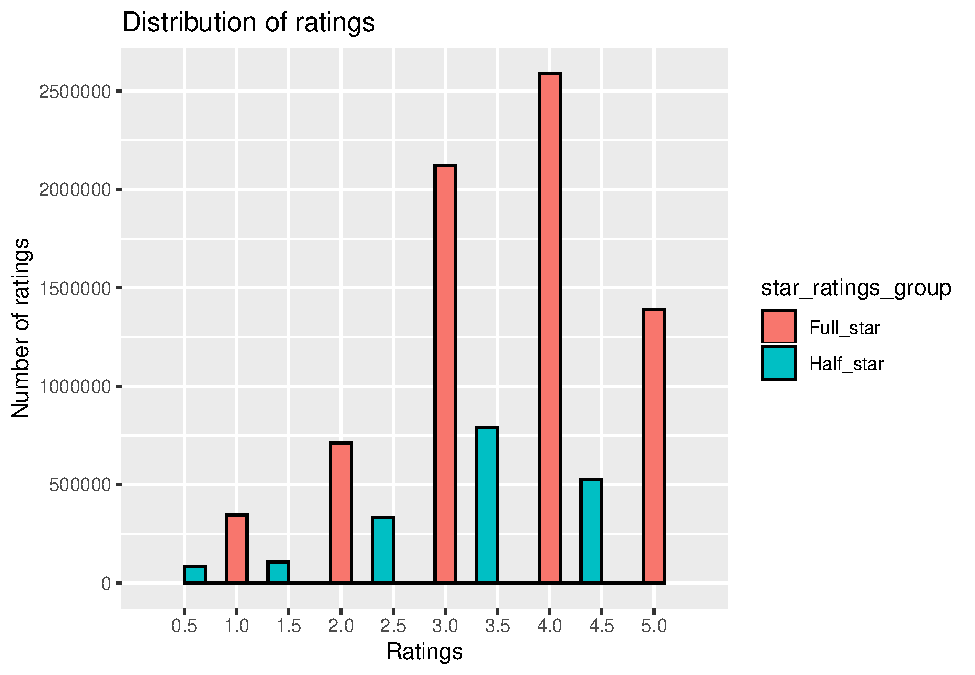
\includegraphics{Project_MovieLens_files/figure-latex/unnamed-chunk-14-1.pdf}

Now, we explore the top 10 and bottom 10 movies based on total number of
ratings. We see that some movies are rated more often than the others.
For instance, 120 movies are rated by one user only.

Top 10 movies are well-known and are rated by many users. But, the
bottom 10 movies appear to be obscure and are only rated by one user.
Therefore, the predictions of future ratings for such movies will be
difficult.

This information is important for our model because a very low rating
numbers can result in overfitting for our predictions. Therefore, the
use of regularization by including this information as a penalty term in
our model (if needed) can improve the RMSE of our model.

\begin{Shaded}
\begin{Highlighting}[]
\NormalTok{movies_count<-(edx }\OperatorTok
\StringTok{  }\KeywordTok{group_by}\NormalTok{(title) }\OperatorTok\KeywordTok{summarize}\NormalTok{(}\DataTypeTok{count=}\KeywordTok{n}\NormalTok{()))}


\KeywordTok{sprintf}\NormalTok{(}\StringTok{"Movies with a single rating = %d"}\NormalTok{,}\KeywordTok{sum}\NormalTok{(movies_count}\OperatorTok{$}\NormalTok{count}\OperatorTok{==}\DecValTok{1}\NormalTok{))}
\end{Highlighting}
\end{Shaded}

\begin{verbatim}
## [1] "Movies with a single rating = 125"
\end{verbatim}

\begin{Shaded}
\begin{Highlighting}[]
\NormalTok{top_movies <-}\StringTok{ }\NormalTok{edx }\OperatorTok
\StringTok{  }\KeywordTok{group_by}\NormalTok{(title) }\OperatorTok
\StringTok{  }\KeywordTok{summarize}\NormalTok{(}\DataTypeTok{count=}\KeywordTok{n}\NormalTok{()) }\OperatorTok
\StringTok{  }\KeywordTok{top_n}\NormalTok{(}\DecValTok{10}\NormalTok{) }\OperatorTok
\StringTok{  }\KeywordTok{arrange}\NormalTok{(}\KeywordTok{desc}\NormalTok{(count))}
\end{Highlighting}
\end{Shaded}

\begin{verbatim}
## Selecting by count
\end{verbatim}

\begin{Shaded}
\begin{Highlighting}[]
\NormalTok{top_movies }\OperatorTok\StringTok{ }
\StringTok{  }\KeywordTok{ggplot}\NormalTok{(}\KeywordTok{aes}\NormalTok{(}\DataTypeTok{x=}\KeywordTok{reorder}\NormalTok{(title, count), }\DataTypeTok{y=}\NormalTok{count)) }\OperatorTok{+}
\StringTok{  }\KeywordTok{geom_bar}\NormalTok{(}\DataTypeTok{stat=}\StringTok{'identity'}\NormalTok{, }\DataTypeTok{fill=}\StringTok{"cadetblue"}\NormalTok{) }\OperatorTok{+}\StringTok{ }\KeywordTok{coord_flip}\NormalTok{(}\DataTypeTok{y=}\KeywordTok{c}\NormalTok{(}\DecValTok{0}\NormalTok{, }\DecValTok{40000}\NormalTok{)) }\OperatorTok{+}
\StringTok{  }\KeywordTok{labs}\NormalTok{(}\DataTypeTok{x=}\StringTok{""}\NormalTok{, }\DataTypeTok{y=}\StringTok{"Number of ratings"}\NormalTok{) }\OperatorTok{+}
\StringTok{  }\KeywordTok{geom_text}\NormalTok{(}\KeywordTok{aes}\NormalTok{(}\DataTypeTok{label=}\NormalTok{ count), }\DataTypeTok{hjust=}\OperatorTok{-}\FloatTok{0.1}\NormalTok{, }\DataTypeTok{size=}\DecValTok{3}\NormalTok{) }\OperatorTok{+}
\StringTok{  }\KeywordTok{labs}\NormalTok{(}\DataTypeTok{title=}\StringTok{"Top 10 movies titles based on number of ratings"}\NormalTok{ )}
\end{Highlighting}
\end{Shaded}

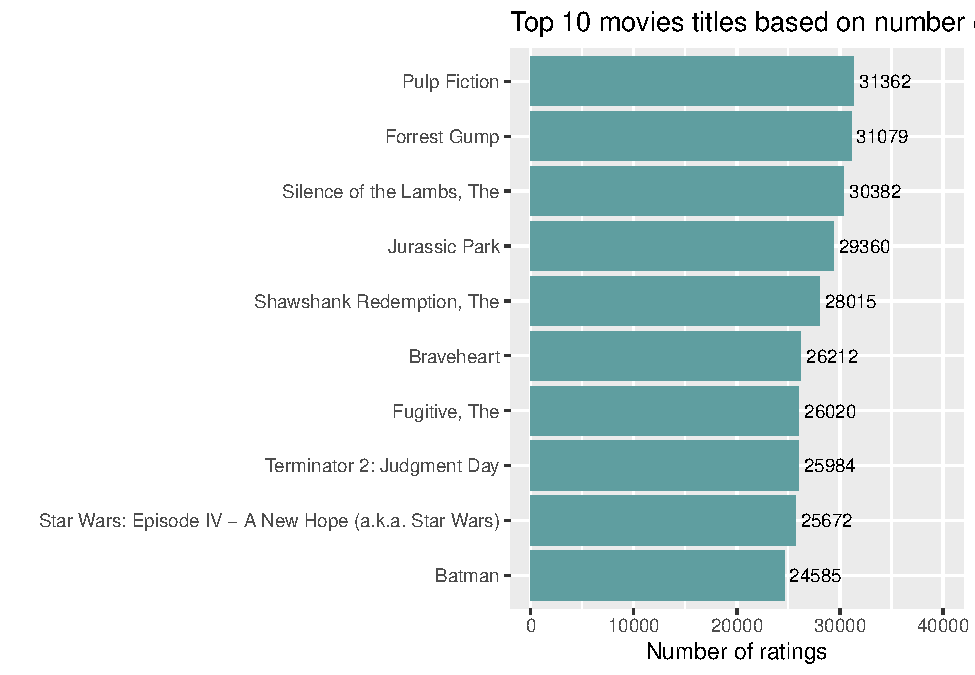
\includegraphics{Project_MovieLens_files/figure-latex/unnamed-chunk-16-1.pdf}

\begin{Shaded}
\begin{Highlighting}[]
\NormalTok{bottom_movies <-}\StringTok{ }\NormalTok{edx }\OperatorTok
\StringTok{  }\KeywordTok{group_by}\NormalTok{(title) }\OperatorTok
\StringTok{  }\KeywordTok{summarize}\NormalTok{(}\DataTypeTok{count=}\KeywordTok{n}\NormalTok{()) }\OperatorTok
\StringTok{  }\KeywordTok{arrange}\NormalTok{(}\KeywordTok{desc}\NormalTok{(count))}

\NormalTok{bottom_movies }\OperatorTok\StringTok{ }\KeywordTok{tail}\NormalTok{(}\DecValTok{10}\NormalTok{) }\OperatorTok
\StringTok{  }\KeywordTok{ggplot}\NormalTok{(}\KeywordTok{aes}\NormalTok{(}\DataTypeTok{x=}\KeywordTok{reorder}\NormalTok{(title, count), }\DataTypeTok{y=}\NormalTok{count)) }\OperatorTok{+}
\StringTok{  }\KeywordTok{geom_bar}\NormalTok{(}\DataTypeTok{stat=}\StringTok{'identity'}\NormalTok{, }\DataTypeTok{fill=}\StringTok{"cadetblue"}\NormalTok{) }\OperatorTok{+}\StringTok{ }\KeywordTok{coord_flip}\NormalTok{(}\DataTypeTok{y=}\KeywordTok{c}\NormalTok{(}\DecValTok{0}\NormalTok{, }\DecValTok{100}\NormalTok{)) }\OperatorTok{+}
\StringTok{  }\KeywordTok{labs}\NormalTok{(}\DataTypeTok{x=}\StringTok{""}\NormalTok{, }\DataTypeTok{y=}\StringTok{"Number of ratings"}\NormalTok{) }\OperatorTok{+}
\StringTok{  }\KeywordTok{geom_text}\NormalTok{(}\KeywordTok{aes}\NormalTok{(}\DataTypeTok{label=}\NormalTok{ count), }\DataTypeTok{hjust=}\OperatorTok{-}\FloatTok{0.1}\NormalTok{, }\DataTypeTok{size=}\DecValTok{3}\NormalTok{) }\OperatorTok{+}
\StringTok{  }\KeywordTok{labs}\NormalTok{(}\DataTypeTok{title=}\StringTok{"Bottom 10 movies based on number of ratings"}\NormalTok{)}
\end{Highlighting}
\end{Shaded}

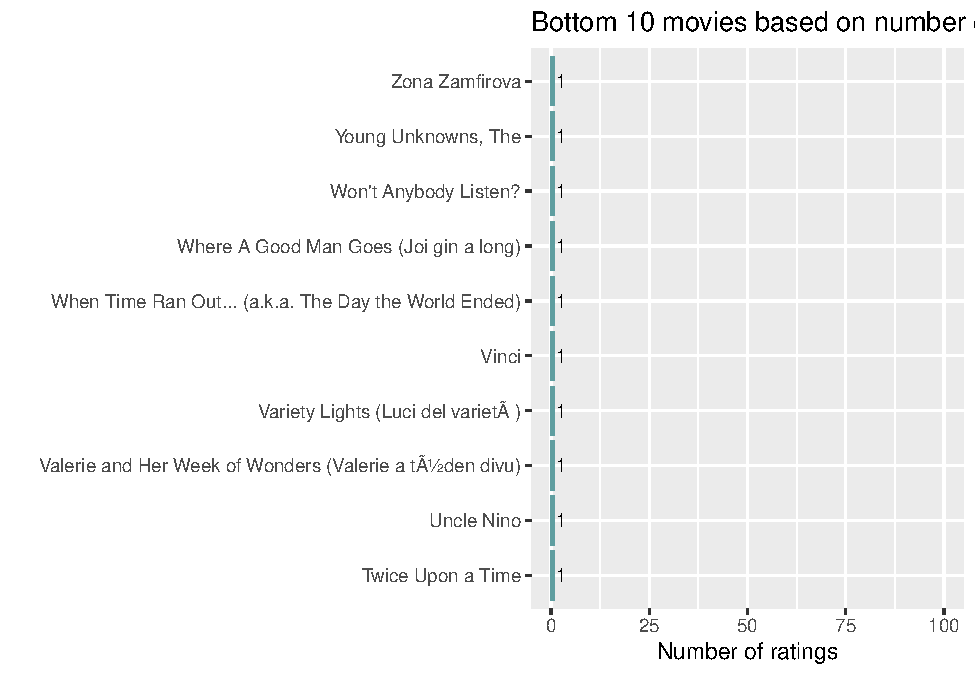
\includegraphics{Project_MovieLens_files/figure-latex/unnamed-chunk-17-1.pdf}

\subsection{Generes}
\label{sec:generes}

Most movies belong to Drama and Comedy generes.A very few movies belong
to horror genere. Though, this information does not add much compared to
previous features. Therefore, we will not use ``genere" feature for our
model building.

\begin{Shaded}
\begin{Highlighting}[]
\NormalTok{generes <-}\StringTok{ }\KeywordTok{c}\NormalTok{(}\StringTok{"Drama"}\NormalTok{,}\StringTok{"Comedy"}\NormalTok{,}\StringTok{"Thriller"}\NormalTok{,}\StringTok{"Romance"}\NormalTok{,}\StringTok{"Sci-Fi"}\NormalTok{,}\StringTok{"Adventure"}\NormalTok{,}\StringTok{"War"}\NormalTok{,}\StringTok{"Action"}\NormalTok{,}\StringTok{"Horror"}\NormalTok{)}
\KeywordTok{sapply}\NormalTok{(generes, }\ControlFlowTok{function}\NormalTok{(x)}
\NormalTok{\{}
 \KeywordTok{sprintf}\NormalTok{(}\StringTok{"%s = %d"}\NormalTok{,x,}\KeywordTok{sum}\NormalTok{(}\KeywordTok{grepl}\NormalTok{(x,edx}\OperatorTok{$}\NormalTok{genres))) }
\NormalTok{\}}
\NormalTok{)}
\end{Highlighting}
\end{Shaded}

\begin{verbatim}
##                 Drama                Comedy              Thriller 
##     "Drama = 3910127"    "Comedy = 3540930"  "Thriller = 2325899" 
##               Romance                Sci-Fi             Adventure 
##   "Romance = 1712100"    "Sci-Fi = 1341183" "Adventure = 1908892" 
##                   War                Action                Horror 
##        "War = 511147"    "Action = 2560545"     "Horror = 691485"
\end{verbatim}

\subsection{Premier Year}
\label{sec:pyear}

We analyse the rating trends of users over the years. Interestingly, we
can see that mean ratings have dropped over the years. This indicates
that users are not rating more movies in recent years.

\begin{Shaded}
\begin{Highlighting}[]
\NormalTok{edx }\OperatorTok\StringTok{ }\KeywordTok{group_by}\NormalTok{(premiereYr) }\OperatorTok
\StringTok{  }\KeywordTok{summarize}\NormalTok{(}\DataTypeTok{rating =} \KeywordTok{mean}\NormalTok{(rating)) }\OperatorTok
\StringTok{  }\KeywordTok{ggplot}\NormalTok{(}\KeywordTok{aes}\NormalTok{(premiereYr, rating)) }\OperatorTok{+}
\StringTok{  }\KeywordTok{geom_point}\NormalTok{() }\OperatorTok{+}
\StringTok{  }\KeywordTok{geom_smooth}\NormalTok{(}\DataTypeTok{alpha=}\FloatTok{0.5}\NormalTok{, }\DataTypeTok{color=}\StringTok{'cadetblue'}\NormalTok{,}\DataTypeTok{method =}\NormalTok{ lm,}\DataTypeTok{formula =}\NormalTok{ y }\OperatorTok{~}\StringTok{ }\NormalTok{splines}\OperatorTok{::}\KeywordTok{bs}\NormalTok{(x, }\DecValTok{3}\NormalTok{))}
\end{Highlighting}
\end{Shaded}

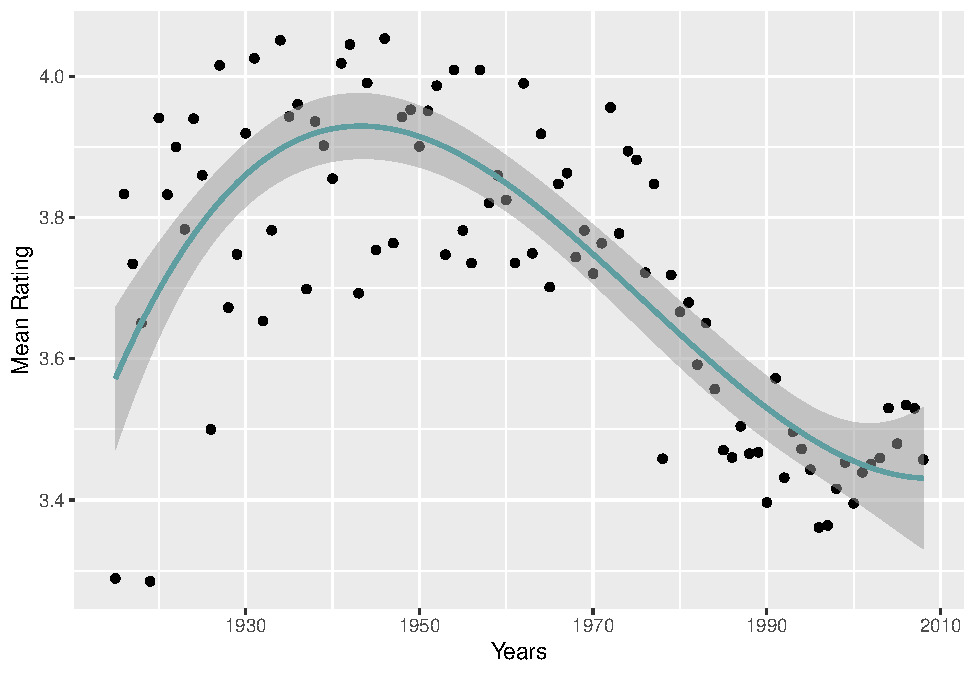
\includegraphics{Project_MovieLens_files/figure-latex/unnamed-chunk-19-1.pdf}

\section{Methods}
\label{sec:methods}

We will use RMSE to estimate the quality of our model. Using equation
\ref{eq:rmse}, we write the following function to compute the RMSE
between actual ratings and predicted ratings::

\begin{Shaded}
\begin{Highlighting}[]
\NormalTok{RMSE <-}\StringTok{ }\ControlFlowTok{function}\NormalTok{(true_ratings, predicted_ratings)\{}
  \KeywordTok{sqrt}\NormalTok{(}\KeywordTok{mean}\NormalTok{((true_ratings }\OperatorTok{-}\StringTok{ }\NormalTok{predicted_ratings)}\OperatorTok{^}\DecValTok{2}\NormalTok{))}
\NormalTok{\}}
\end{Highlighting}
\end{Shaded}

The lower RMSE is better.The evaluation criteria for this project is
that RMSE of the proposed model should be less than 0.8649.

\begin{Shaded}
\begin{Highlighting}[]
\CommentTok{#Initiate RMSE results to compare various models}
\NormalTok{rmse_results <-}\StringTok{ }\KeywordTok{data_frame}\NormalTok{(}\DataTypeTok{method =} \StringTok{"Target RSME"}\NormalTok{, }\DataTypeTok{RMSE =} \FloatTok{0.8649}\NormalTok{)}
\end{Highlighting}
\end{Shaded}

\begin{verbatim}
## Warning: `data_frame()` is deprecated, use `tibble()`.
## This warning is displayed once per session.
\end{verbatim}

\begin{Shaded}
\begin{Highlighting}[]
\NormalTok{rmse_results}
\end{Highlighting}
\end{Shaded}

\begin{longtable}[]{@{}lr@{}}
\toprule
method & RMSE\tabularnewline
\midrule
\endhead
Target RSME & 0.8649\tabularnewline
\bottomrule
\end{longtable}

\subsection{Average Movie Rating Model}
\label{sec:am}

We start with the simplest model by predicting the same ratings for all
movies regardless of users or freqeuncy of ratings. In other words, we
compute the dataset's mean raitng as follows:

\begin{equation}
Y_{u, i} = \mu + \epsilon_{u, i}
\end{equation}

Where \(\epsilon_{u,i}\) is the independent error sample from the same
distribution centered at 0 and \(\mu\) the ``true" rating for all
movies. This model is based on the assumption that differences in movie
ratings can be explained by random variation alone. The expected value
of the data is around 3.5 and we obtain a RMSE of 1.06.

\begin{Shaded}
\begin{Highlighting}[]
\CommentTok{# Calculating mean of ratings}
\NormalTok{mu <-}\StringTok{ }\KeywordTok{mean}\NormalTok{(edx}\OperatorTok{$}\NormalTok{rating)}
\NormalTok{mu}
\end{Highlighting}
\end{Shaded}

\begin{verbatim}
## [1] 3.512465
\end{verbatim}

We make predictions using \(\mu\) and obtain our firt RMSE score of
1.06.

\begin{Shaded}
\begin{Highlighting}[]
\CommentTok{# Making predictions using mean rating}
\NormalTok{naive_rmse <-}\StringTok{ }\KeywordTok{RMSE}\NormalTok{(validation}\OperatorTok{$}\NormalTok{rating, mu)}
\NormalTok{rmse_results <-}\StringTok{ }\KeywordTok{bind_rows}\NormalTok{(rmse_results,}
                          \KeywordTok{data_frame}\NormalTok{(}\DataTypeTok{method=}\StringTok{"Average Rating Model"}\NormalTok{,  }
                                     \DataTypeTok{RMSE =}\NormalTok{ naive_rmse ))}
\NormalTok{rmse_results}
\end{Highlighting}
\end{Shaded}

\begin{longtable}[]{@{}lr@{}}
\toprule
method & RMSE\tabularnewline
\midrule
\endhead
Target RSME & 0.864900\tabularnewline
Average Rating Model & 1.061202\tabularnewline
\bottomrule
\end{longtable}

In order to improve the RMSE of our model, we have to include extra
parameters in our model. We can use some of the insights obtained in
previous section, such as user effect.

\subsection{Movie Effect Model}
\label{sec:mem}

We recall from Section \ref{sec:dataanalsyis} that different movies are
rated differently. The popular movies are rated much higher than
unpopular movies. We can modify our previous model by adding the term
`\(b_{i}\)" to represent average ranking for movie i as follows:

\begin{equation}
Y_{u, i} = \mu +b_{i}+ \epsilon_{u, i}
\end{equation}

The least squares estimate \(b_{i}\) is just the average of
\(Y_{u,i} - \mu\) for each movie \(i\). So we can compute it as follows:

\begin{Shaded}
\begin{Highlighting}[]
\NormalTok{mu <-}\StringTok{ }\KeywordTok{mean}\NormalTok{(edx}\OperatorTok{$}\NormalTok{rating)}
\NormalTok{movie_avgs <-}\StringTok{ }\NormalTok{edx }\OperatorTok
\StringTok{  }\KeywordTok{group_by}\NormalTok{(movieId) }\OperatorTok
\StringTok{  }\KeywordTok{summarize}\NormalTok{(}\DataTypeTok{b_i =} \KeywordTok{mean}\NormalTok{(rating }\OperatorTok{-}\StringTok{ }\NormalTok{mu))}
\end{Highlighting}
\end{Shaded}

The histogram is skewed to the left, which implies that most movies have
negative effects. This is known as penalty term movie effect.

\begin{Shaded}
\begin{Highlighting}[]
\NormalTok{movie_avgs}\OperatorTok
\KeywordTok{ggplot}\NormalTok{(}\KeywordTok{aes}\NormalTok{(b_i)) }\OperatorTok{+}
\KeywordTok{geom_histogram}\NormalTok{(}\DataTypeTok{bins =} \DecValTok{30}\NormalTok{, }\DataTypeTok{color =} \StringTok{"black"}\NormalTok{)}
\end{Highlighting}
\end{Shaded}

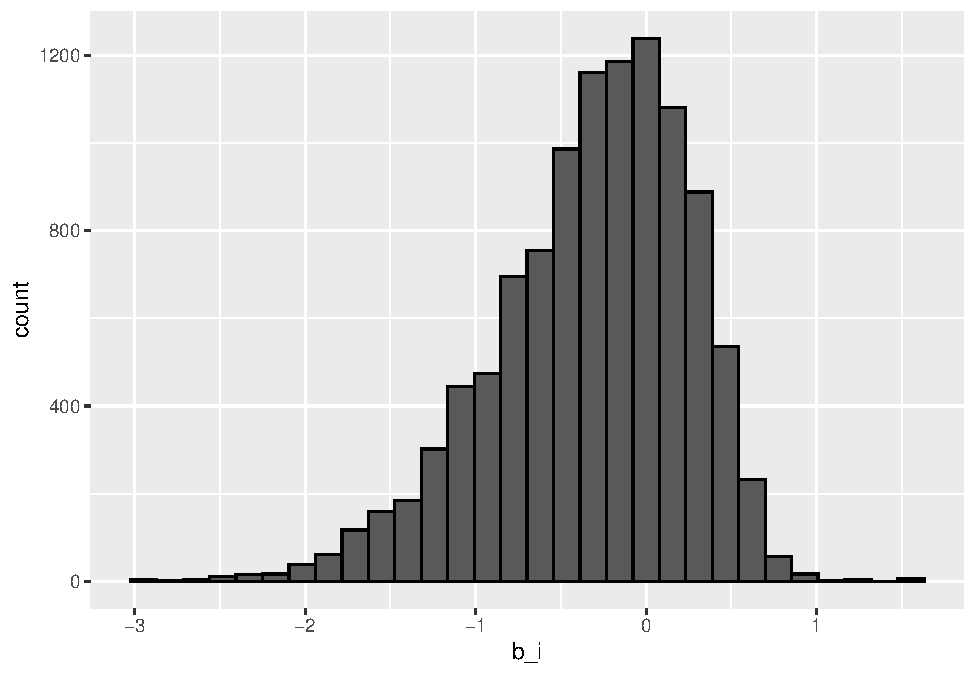
\includegraphics{Project_MovieLens_files/figure-latex/unnamed-chunk-25-1.pdf}
If one movie is on average rated worse than the average rating of all
movies \(\mu\), then we predict that it will rated lower that \(\mu\) by
\(b_{i}\).By including the movie effect, our model's RMSE improves to
0.9437 on validation data.

\begin{Shaded}
\begin{Highlighting}[]
\NormalTok{predicted_ratings <-}\StringTok{ }\NormalTok{mu }\OperatorTok{+}\StringTok{  }\NormalTok{validation }\OperatorTok
\StringTok{  }\KeywordTok{left_join}\NormalTok{(movie_avgs, }\DataTypeTok{by=}\StringTok{'movieId'}\NormalTok{) }\OperatorTok
\StringTok{  }\KeywordTok{pull}\NormalTok{(b_i)}
\NormalTok{model_}\DecValTok{1}\NormalTok{_rmse <-}\StringTok{ }\KeywordTok{RMSE}\NormalTok{(predicted_ratings, validation}\OperatorTok{$}\NormalTok{rating)}
\NormalTok{rmse_results <-}\StringTok{ }\KeywordTok{bind_rows}\NormalTok{(rmse_results,}
                          \KeywordTok{data_frame}\NormalTok{(}\DataTypeTok{method=}\StringTok{"Movie effect model"}\NormalTok{,  }
                                     \DataTypeTok{RMSE =}\NormalTok{ model_}\DecValTok{1}\NormalTok{_rmse ))}
\NormalTok{rmse_results}
\end{Highlighting}
\end{Shaded}

\begin{longtable}[]{@{}lr@{}}
\toprule
method & RMSE\tabularnewline
\midrule
\endhead
Target RSME & 0.8649000\tabularnewline
Average Rating Model & 1.0612018\tabularnewline
Movie effect model & 0.9439087\tabularnewline
\bottomrule
\end{longtable}

\section{User Effects}
\label{sec:ue}

We know that some users are more active than others.We compute the
average rating for user \(\mu\), for those that have rated over 50
movies. There is also substantial variability acorss users. Some users
are very cranky (like few movies), and other users love every movie.
Therefore, we can further improve our previous model by adding
user-specific effect (\(b_{u}\)):

\begin{equation}
Y_{u, i} = \mu + b_{i} + b_{u} + \epsilon_{u, i}
\end{equation}

\begin{Shaded}
\begin{Highlighting}[]
\NormalTok{edx }\OperatorTok\StringTok{ }
\StringTok{  }\KeywordTok{left_join}\NormalTok{(movie_avgs, }\DataTypeTok{by=}\StringTok{'movieId'}\NormalTok{) }\OperatorTok
\StringTok{  }\KeywordTok{group_by}\NormalTok{(userId) }\OperatorTok
\StringTok{  }\KeywordTok{filter}\NormalTok{(}\KeywordTok{n}\NormalTok{() }\OperatorTok{>=}\StringTok{ }\DecValTok{100}\NormalTok{) }\OperatorTok
\StringTok{  }\KeywordTok{summarize}\NormalTok{(}\DataTypeTok{b_u =} \KeywordTok{mean}\NormalTok{(rating }\OperatorTok{-}\StringTok{ }\NormalTok{mu }\OperatorTok{-}\StringTok{ }\NormalTok{b_i)) }\OperatorTok
\StringTok{  }\KeywordTok{ggplot}\NormalTok{(}\KeywordTok{aes}\NormalTok{(b_u)) }\OperatorTok{+}
\StringTok{  }\KeywordTok{geom_histogram}\NormalTok{(}\DataTypeTok{bins =} \DecValTok{10}\NormalTok{, }\DataTypeTok{color =} \StringTok{"black"}\NormalTok{)}
\end{Highlighting}
\end{Shaded}

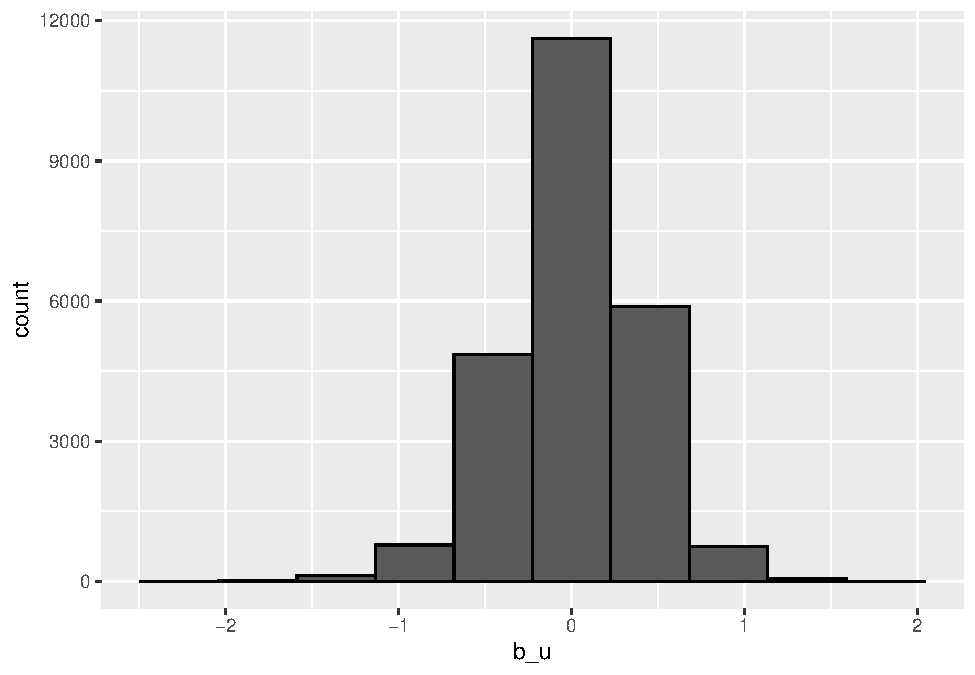
\includegraphics{Project_MovieLens_files/figure-latex/unnamed-chunk-27-1.pdf}

If a cranky user (negative \(b_{u}\)) rates a great movie (positive
\(b_{i}\)), the effects counter each other. And, we may be able to
correctly predict that this user gave this great movie a 3 rather than a
5. We estimate \(b_{u}\) as the average of \[Y_{u, i} - \mu - b_{i}\] as
shown below.

\begin{Shaded}
\begin{Highlighting}[]
\NormalTok{user_avgs <-}\StringTok{ }\NormalTok{edx }\OperatorTok
\KeywordTok{left_join}\NormalTok{(movie_avgs, }\DataTypeTok{by=}\StringTok{'movieId'}\NormalTok{) }\OperatorTok
\KeywordTok{group_by}\NormalTok{(userId) }\OperatorTok
\KeywordTok{summarize}\NormalTok{(}\DataTypeTok{b_u =} \KeywordTok{mean}\NormalTok{(rating }\OperatorTok{-}\StringTok{ }\NormalTok{mu }\OperatorTok{-}\StringTok{ }\NormalTok{b_i))}
\end{Highlighting}
\end{Shaded}

By using new model for prediction, the RMSE improves to 0.865.

\begin{Shaded}
\begin{Highlighting}[]
\NormalTok{predicted_ratings <-}\StringTok{ }\NormalTok{validation}\OperatorTok
\StringTok{  }\KeywordTok{left_join}\NormalTok{(movie_avgs, }\DataTypeTok{by=}\StringTok{'movieId'}\NormalTok{) }\OperatorTok
\StringTok{  }\KeywordTok{left_join}\NormalTok{(user_avgs, }\DataTypeTok{by=}\StringTok{'userId'}\NormalTok{) }\OperatorTok
\StringTok{  }\KeywordTok{mutate}\NormalTok{(}\DataTypeTok{pred =}\NormalTok{ mu }\OperatorTok{+}\StringTok{ }\NormalTok{b_i }\OperatorTok{+}\StringTok{ }\NormalTok{b_u) }\OperatorTok
\StringTok{  }\KeywordTok{pull}\NormalTok{(pred)}
\NormalTok{model_}\DecValTok{2}\NormalTok{_rmse <-}\StringTok{ }\KeywordTok{RMSE}\NormalTok{(predicted_ratings, validation}\OperatorTok{$}\NormalTok{rating)}
\NormalTok{rmse_results <-}\StringTok{ }\KeywordTok{bind_rows}\NormalTok{(rmse_results,}
                          \KeywordTok{data_frame}\NormalTok{(}\DataTypeTok{method=}\StringTok{"Movie and user effect model"}\NormalTok{,  }
                                     \DataTypeTok{RMSE =}\NormalTok{ model_}\DecValTok{2}\NormalTok{_rmse))}
\NormalTok{rmse_results}
\end{Highlighting}
\end{Shaded}

\begin{longtable}[]{@{}lr@{}}
\toprule
method & RMSE\tabularnewline
\midrule
\endhead
Target RSME & 0.8649000\tabularnewline
Average Rating Model & 1.0612018\tabularnewline
Movie effect model & 0.9439087\tabularnewline
Movie and user effect model & 0.8653488\tabularnewline
\bottomrule
\end{longtable}

\subsection{Regularization Using Moives and Users}
\subsection{sec:reg}

There is still room for improvement as we stil made mistakes on our
first model (using only movies). There are users who have rated very few
movies (less than 30 movies). On the other hand, some movies are rated
very few times (say 1 or 2). These are basically noisy estimates that
result in overfitting of the model. Such large errors are likely
increase the RMSE and affect our predictions.

To tackle this problem, we use the concept of regularization. The
regularization permits to penalize large estimates that come from small
sample sizes. First, we find the value of lambda (that is a tuning
parameter) that will minimize the RMSE.

\begin{Shaded}
\begin{Highlighting}[]
\KeywordTok{library}\NormalTok{(tidyverse)}
\NormalTok{lambdas <-}\StringTok{ }\KeywordTok{seq}\NormalTok{(}\DecValTok{0}\NormalTok{, }\DecValTok{10}\NormalTok{, }\FloatTok{0.25}\NormalTok{)}
\NormalTok{rmses <-}\StringTok{ }\KeywordTok{sapply}\NormalTok{(lambdas, }\ControlFlowTok{function}\NormalTok{(l)\{}
  
\NormalTok{  mu <-}\StringTok{ }\KeywordTok{mean}\NormalTok{(edx}\OperatorTok{$}\NormalTok{rating)}
  
\NormalTok{  b_i <-}\StringTok{ }\NormalTok{edx }\OperatorTok\StringTok{ }
\StringTok{    }\KeywordTok{group_by}\NormalTok{(movieId) }\OperatorTok
\StringTok{    }\KeywordTok{summarize}\NormalTok{(}\DataTypeTok{b_i =} \KeywordTok{sum}\NormalTok{(rating }\OperatorTok{-}\StringTok{ }\NormalTok{mu)}\OperatorTok{/}\NormalTok{(}\KeywordTok{n}\NormalTok{()}\OperatorTok{+}\NormalTok{l))}
  
\NormalTok{  b_u <-}\StringTok{ }\NormalTok{edx }\OperatorTok\StringTok{ }
\StringTok{    }\KeywordTok{left_join}\NormalTok{(b_i, }\DataTypeTok{by=}\StringTok{"movieId"}\NormalTok{) }\OperatorTok
\StringTok{    }\KeywordTok{group_by}\NormalTok{(userId) }\OperatorTok
\StringTok{    }\KeywordTok{summarize}\NormalTok{(}\DataTypeTok{b_u =} \KeywordTok{sum}\NormalTok{(rating }\OperatorTok{-}\StringTok{ }\NormalTok{b_i }\OperatorTok{-}\StringTok{ }\NormalTok{mu)}\OperatorTok{/}\NormalTok{(}\KeywordTok{n}\NormalTok{()}\OperatorTok{+}\NormalTok{l))}
  
\NormalTok{  predicted_ratings <-}\StringTok{ }
\StringTok{    }\NormalTok{validation }\OperatorTok\StringTok{ }
\StringTok{    }\KeywordTok{left_join}\NormalTok{(b_i, }\DataTypeTok{by =} \StringTok{"movieId"}\NormalTok{) }\OperatorTok
\StringTok{    }\KeywordTok{left_join}\NormalTok{(b_u, }\DataTypeTok{by =} \StringTok{"userId"}\NormalTok{) }\OperatorTok
\StringTok{    }\KeywordTok{mutate}\NormalTok{(}\DataTypeTok{pred =}\NormalTok{ mu }\OperatorTok{+}\StringTok{ }\NormalTok{b_i }\OperatorTok{+}\StringTok{ }\NormalTok{b_u) }\OperatorTok
\StringTok{    }\KeywordTok{pull}\NormalTok{(pred)}
  
  \KeywordTok{return}\NormalTok{(}\KeywordTok{RMSE}\NormalTok{(predicted_ratings, validation}\OperatorTok{$}\NormalTok{rating))}
\NormalTok{\})}
\end{Highlighting}
\end{Shaded}

We can see that the optimal lambda value is 5.25, which gives us a RMSE
of 0.8649.

\begin{Shaded}
\begin{Highlighting}[]
\KeywordTok{qplot}\NormalTok{(lambdas, rmses)  }
\end{Highlighting}
\end{Shaded}

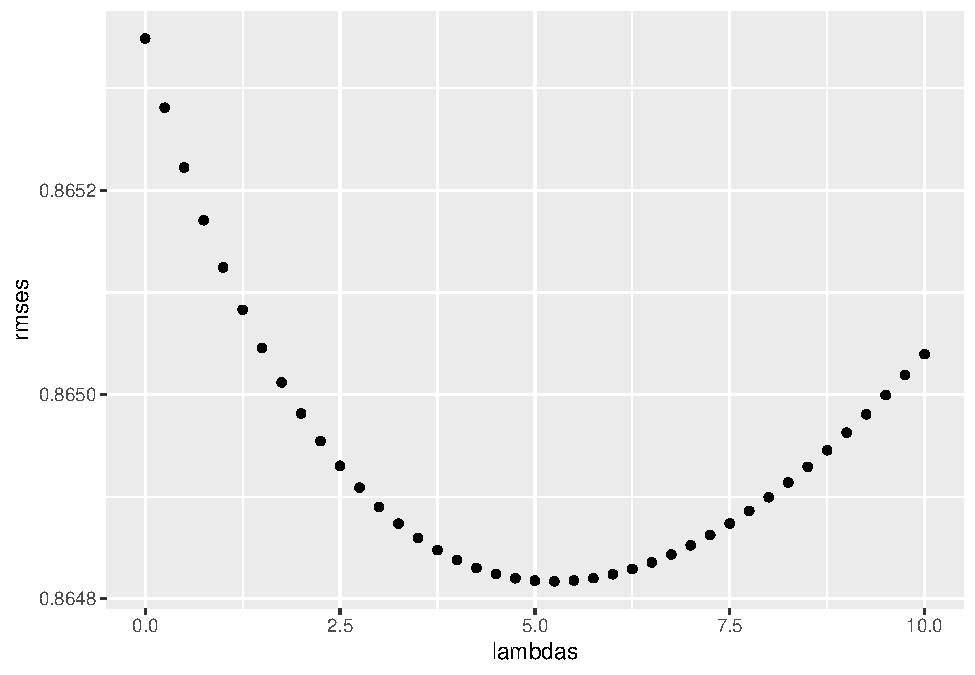
\includegraphics{Project_MovieLens_files/figure-latex/plot_lambdas-1.pdf}

\begin{Shaded}
\begin{Highlighting}[]
\NormalTok{lambda <-}\StringTok{ }\NormalTok{lambdas[}\KeywordTok{which.min}\NormalTok{(rmses)]}
\NormalTok{lambda}
\end{Highlighting}
\end{Shaded}

\begin{verbatim}
## [1] 5.25
\end{verbatim}

\begin{Shaded}
\begin{Highlighting}[]
\NormalTok{rmse_results <-}\StringTok{ }\KeywordTok{bind_rows}\NormalTok{(rmse_results,}
                          \KeywordTok{data_frame}\NormalTok{(}\DataTypeTok{method=}\StringTok{"Regularized movie and user effect model"}\NormalTok{,  }
                                     \DataTypeTok{RMSE =} \KeywordTok{min}\NormalTok{(rmses)))}
\NormalTok{rmse_results}
\end{Highlighting}
\end{Shaded}

\begin{longtable}[]{@{}lr@{}}
\toprule
method & RMSE\tabularnewline
\midrule
\endhead
Target RSME & 0.8649000\tabularnewline
Average Rating Model & 1.0612018\tabularnewline
Movie effect model & 0.9439087\tabularnewline
Movie and user effect model & 0.8653488\tabularnewline
Regularized movie and user effect model & 0.8648170\tabularnewline
\bottomrule
\end{longtable}

\section{Results}
\label{sec:results}

We can analyse the RMSEs for the various models trained in the previouse
section. We started with a very basic approach of predicting the mean
ratingregardless of the user. Then, we added movie and user effects to
the simple model. Finally, we experimented regularization with movie and
user effects. For regularization, we found the optimal value of turing
parameter lambda.The resultant RMSEs are as follows:

\begin{Shaded}
\begin{Highlighting}[]
\NormalTok{rmse_results}
\end{Highlighting}
\end{Shaded}

\begin{longtable}[]{@{}lr@{}}
\toprule
method & RMSE\tabularnewline
\midrule
\endhead
Target RSME & 0.8649000\tabularnewline
Average Rating Model & 1.0612018\tabularnewline
Movie effect model & 0.9439087\tabularnewline
Movie and user effect model & 0.8653488\tabularnewline
Regularized movie and user effect model & 0.8648170\tabularnewline
\bottomrule
\end{longtable}

We can see that the RMSE of our final model is 0.864817. This is a
significant improvement (decrease in RMSE of around 18.5\%) compared to
the first simple model.

\section{Conclusion}
\label{sec:conclusion}

The simplest model which predicts the same rating (mean rating) for all
movies regardless of user gave anRMSE above 1. If RMSE is larger than 1,
it means our typical error is larger than one star, which is notgood. By
taking into consideration the movie effect the RMSE went down to
0.9439087 which was a greatimprovement. RMSE further went down to
0.8653488 after modelling the user effect in the previous model.However,
the lowest RMSE i.e, 0.8648201 was achieved by regularizing the movie
and user effect, whichpenalized larger estimates of ratings from
relatively small sample size of users.Subsequently, regularizing the
year and genres effects can further improve the residual mean squared
errorbut regularizing the genres is computationally very expensive since
it requires separating multiple genres formany movies into multiple
observations for a given movie i having single genre in genres column.

In this report we described a way to build up the recommendation
algorithm to predict movie ratings using Movielens data set step by
step. Four predictors were used in our algorithm included: (i) the
baseline as average rating of each movie, (ii) the specific-effect by
user, (iii) the specific-effect by aging time, (iv) the specific-effect
by genres. Two main predictors have highest impact to the results are
the average rating of each movie and the specific-effect by user. The
final RMSE from our algorithm is 0.8645. This result achieved our
project goals and the initial criteria of the course HarvardX - PH125.9X
Data Science: Capstone project - All learners (RMSE \textless{}
0.8649).Because our algorithm is based on the average rating of each
movie, therefore if a movie have very less number of rating, this
algorithm is limited to provide an accuracy results. A better result is
received only when the number of rating of a movie and/or the number of
rating given by a user is increased high enough.However this is an
opportunity to improve our algorithm in the future by including the
number of rating of a movie and the number of rating given by a user to
our algorithm. Furthermore, other machine learning techniques such as
Regularization, Penalized Least Squares, Matrix Factorization could also
improve the results further.Another limitation during this project time
is the hardware, especially RAM as the main constraint, and the speed of
normal laptop.

\begin{Shaded}
\begin{Highlighting}[]
\NormalTok{rmse_results}
\end{Highlighting}
\end{Shaded}

\begin{longtable}[]{@{}lr@{}}
\toprule
method & RMSE\tabularnewline
\midrule
\endhead
Target RSME & 0.8649000\tabularnewline
Average Rating Model & 1.0612018\tabularnewline
Movie effect model & 0.9439087\tabularnewline
Movie and user effect model & 0.8653488\tabularnewline
Regularized movie and user effect model & 0.8648170\tabularnewline
\bottomrule
\end{longtable}

\begin{thebibliography}{9}
\bibitem{rsystems} 
Baptiste Rocca -Introduction to recommender systems \url{https://towardsdatascience.com/introduction-to-recommender-systems-6c66cf15ada}
\bibitem{rsystems1}
Resnick, P., Varian, H. \textit{Recommender Systems}. CACM 40(3), 56–58 (1997)
\bibitem{nfc}
Netflix Prize \url{https://en.wikipedia.org/wiki/Netflix_Prize}

\bibitem{dataset}
MovieLens 10M Dataset \url{https://grouplens.org/datasets/movielens/10m}

\bibitem{rmse}
James Moody - What does RMSE really mean? \url{https://towardsdatascience.com/what-does-rmse-really-mean-806b65f2e48e}

\bibitem{rafa}
Rafael Irizarry - Introduction to Data Science \url{https://rafalab.github.io/dsbook}


\end{thebibliography}


\end{document}
